\chapter[$\zmod{2}$ Homology]{Simplicial $\ZZ_2$-Homology: Physical Algebra}
\section{Intro}
This chapter, we'll talk about \emph{homology}, which captures holes in a much
more satisfying way than higher homotopy groups do.
\begin{adjustwidth}{1.5em}{}
  \begin{remark}
    Although not exactly accurate, a good way to start to understand homology for
    a space $X$ is to view an $n$-manifold in $X$ that is not the boundary of an
    $(n+1)$-manifold-with-boundary as capturing some geometry of $X$ while an
    $n$-manifold that is the boundary of an $(n+1)$-dimensional
    manifold-with-boundary is not detecting any hole or structure.
  \end{remark}
\end{adjustwidth}
\section{Chains, Cycles, Boundaries, and the Homology Groups}
\begin{definition}
  An \emph{$n$-chain} of $K$ is a finite formal sum
  \[
    \sum_{i=1}^k \sigma_i
  \]
  of distinct $n$-simplices in $K$. Note that the dimensions of the simplices
  must be the same. So \emph{chain} will mean $n$-chain whenever the dimension
  is either unimportant or understood.
\end{definition}
\begin{definition}
  The \emph{$n$-chain group of $K$} (with coefficients in $\zmod{2}$), denoted
  $\mathsf{C}_n(K)$, is the collection of $n$-chains in $K$ under formal
  addition modulo 2. If there are no $n$-simplices in $K$, the $n$-chain group
  of $K$ is defined to be trivial (containing the ``empty'' chain).
\end{definition}
\begin{problem}[16.1]
  Check that $\msf C_n(K)$ is an abelian group.
\end{problem}
\begin{solution}
  \begin{enumerate}[label=(\arabic*)]
  \item $\epsilon = \sum_{i \in \varnothing} \sigma_i$.
  \item Associativity inherited from $\cup$.
  \item Closure inherited from $\cup$ over the domain given.
  \item Existence of inverses --- since we're taking formal linear
    combinations over $\zmod{2}$, then every element is its own inverse.
  \end{enumerate}
  Finally, to see that $\msf C_n(K)$ is abelian, observe that $+$ in $\msf
  C_n(K)$ inherits commutativity from $\cup$.
\end{solution}
\begin{definition}
  The \emph{$\zmod{2}$-boundary of an $n$-simplex $\sigma = \simp{n}$} is
  defined by
  \[
    \partial \sigma = \sum_{i=0}^n \simpdel{i}{n}
  \]
  the formal sum of the $(n-1)$-faces of $\sigma$.

  For a 0-simplex, the $\zmod{2}$ boundary is defined to be $0 \in \msf
  C_{-1}(K)$.
\end{definition}
\begin{definition}
  The \emph{$\zmod{2}$ boundary of an $n$-chain} is the sum of the boundaries of
  the simplices. That is, $\partial_n : \msf C_n(K) \to \msf C_{n-1}(K)$ is
  given by
  \[
    \partial\pn{\sum_{i=1}^k \sigma_i} = \sum_{i=1}^k \partial(\sigma_i)
  \]
\end{definition}
\begin{problem}[16.2]
  Verify that $\partial$ is a homomorphism, and use the definition to compute
  the $\zmod{2}$ boundary of $\sigma_1 + \sigma_2$ in Figure 16.1
\end{problem}
\begin{solution}
  We want to show $\partial$ is a homomorphism.
  \begin{enumerate}
  \item Let $\epsilon_n \in \msf C_n(K)$ be identity. We want to show
    $\partial(\epsilon_n) = \epsilon_{n-1}$. Taking the empty sum to be
    identity, we see
    \begin{align*}
      \partial(\epsilon_n)
      &=
        \partial\pn{\sum_{i\in \varnothing} \sigma_i} \\
      &= \sum_{i\in\varnothing} \partial\pn{\sigma_i} \\
      &= \epsilon_{n-1}
    \end{align*}
    as desired.
  \item That $\partial$ respects addition is definitional.
  \end{enumerate}
  We have $\partial(\sigma_1 + \sigma_2) = e_1 + e_2 + e_4 + e_5$.
\end{solution}
\begin{definition}
  An \emph{$n$-cycle} is an $n$-chain of $K$ whose boundary is zero. The set of
  all $n$-cycles on $K$ is denoted $\msf Z_n(K)$. An \emph{$n$-boundary} is an
  $n$-chain that is the boundary of an $(n+1)$-chain of $K$. The set of all
  $n$-boundaries is denoted $\msf B_n(K)$.
\end{definition}
% \begin{problem}[16.3]

% \end{problem}
\begin{problem}[16.4]
  Both $\msf Z_n(K)$ and $\msf B_n(K)$ are subgroups of $\msf C_n(K)$. Moreover,
  \[
    \partial \circ \partial = 0.
  \]
  In other words, $\partial_n \circ \partial_{n+1} = 0$ for each index $n \geq
  0$. Hence, $\msf B_n(K) \subset \msf Z_n(K)$.
\end{problem}
\begin{solution}
  Let $\sigma_1, \sigma_2 \in \msf Z_n(K)$. Then by linearity of $\partial_n$,
  we have
  \begin{align*}
    \partial_n(\sigma_1 + \sigma_2)
    &= \partial_n(\sigma_1) + \partial_n(\sigma_2) \\
    &= 0
  \end{align*}
  and hence $\msf Z_n(K) < \msf C_n(K)$.

  Now, let $\sigma_1, \sigma_2 \in \msf B_n(K)$. Then $\exists \tau_1, \tau_2
  \in \msf Z_{n+1}(K)$ such that $\partial_{n+1}(\tau_1) = \sigma_1,
  \partial_{n+1}(\tau_2) = \sigma_{2}$. Since $\msf Z_{n+1}(K) < \msf
  C_{n+1}(K)$, then $\tau_1 + \tau_2 \in \msf Z_{n+1}(K)$. Now, by linearity of
  $\partial$, we have
  \begin{align*}
    \partial_{n+1}(\tau_1 + \tau_2)
    &= \partial_{n+1}(\tau_1) + \partial_{n+1}(\tau_2) \\
    &= \sigma_1 + \sigma_2
  \end{align*}
  hence $\msf B_n(K)$ is a subset closed under the operation, so we have $\msf
  B_n(K) < \msf C_n(K)$.

  It remains to show $\partial_n \circ \partial_{n+1} = 0$. Let $\sigma \in \msf
  C_{n+1}(K)$. Then
  \begin{align*}
    \partial_{n+1}(\sigma)
    &= \partial_{n+1}\pn{\sum_{i \in I} \simp[v^{(i)}]{n+1}} \\
    &= \sum_{i\in I} \partial_{n+1}\pn{\simp[v^{(i)}]{n+1}} \\
    &= \sum_{i\in I} \sum_{j \in [n+1]} \simpdel[v^{(i)}]{j}{n+1}
  \end{align*}
  and so
  \begin{align*}
    \partial_n \pn{\partial_{n+1}(\sigma)}
    &= \sum_{i\in I} \sum_{j \in [n+1]} \partial_{n}\pn{\simpdel[v^{(i)}]{j}{n+1}} \\
    &= \sum_{i\in I} \sum_{j \in [n+1]} \sum_{\substack{k \in [n+1] \\ k \neq j}} \set{v_0^{(i)} \cdots \widehat{v_k^{(i)}} \cdots \widehat{v_j^{(i)}}\cdots v^{(i)}_{n+1}}
  \end{align*}
  hence all the terms cancel, and we're left with $\mb 0$. So $\partial_n \circ
  \partial_{n+1} = 0$, as desired.

  Since every $\sigma \in \msf B_n(K)$ is of the form $\partial_{n+1}(\tau)$
  where $\tau \in \msf C_{n+1}(K)$, it follows that $\partial_n\fim[\msf
  B_n(K)] = (\partial_n \circ \partial_{n+1}) (\msf C_{n+1}(K)) = 0$. Thus $\msf
  B_n(K) < \msf Z_n(K)$.
\end{solution}
\begin{definition}
  Two $n$-cycles $\alpha$ and $\beta$ in $K$ are \emph{equivalent} or
  \emph{homologous} iff $\alpha-\beta = \partial(\gamma)$ for some $(n+1)$-chain
  $\gamma$. In other words, $\alpha$ and $\beta$ are homologous iff they differ
  by an element of the subgroup $\msf B_n(K)$, denoted by
  \[
    \alpha \sim_{\zmod{2}} \beta.
  \]
  The equivalence class of $\alpha$ is denoted by enclosing it in brackets
  thusly: $[\alpha]$. For $\zmod{2}$ $n$-chains, observe that $\alpha - \beta =
  \alpha + \beta$. So we see that two $n$-cycles are equivalent if together they
  bound an $(n+1)$-chain.
\end{definition}
\begin{definition}
  The \emph{$n$\textsuperscript{th}-homology group} (with coefficients in
  $\zmod{2}$) of a finite simplicial complex $K$, denoted $\msf H_n(K)$, is the
  additive group whose elements are equivalence classes of cycles under the
  $\zmod{2}$-equivalence defined above, with $\bk{\alpha} + \bk{\beta} =
  \bk{\alpha +\beta}$. I.e.,
  \[
    \msf H_n(K) = \msf Z_n(K)/\msf B_n(K)
  \]
\end{definition}
\begin{problem}[F1]
  Consider the simplicial complex given below in Figure \ref{fig:F1}. Then for
  $n = 0, 1, 2$,
  \begin{enumerate}
  \item describe elements of $\msf C_n(K)$,
  \item compute $\msf Z_n(K)$,
  \item compute $\msf B_n(K)$, and
  \item compute $\msf H_n(K)$.
  \end{enumerate}
\end{problem}
\begin{figure}[H]
  \centering
  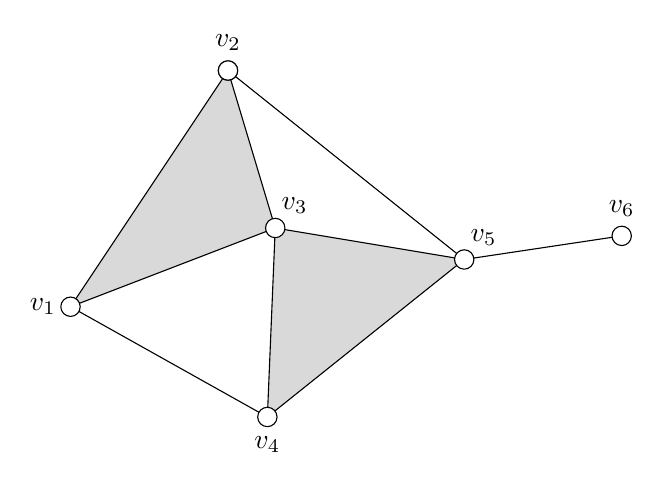
\begin{tikzpicture}[
    every node/.style={
      circle,
      draw=black,
      fill=white,
      inner sep=0pt,
      minimum size=7pt
    }
    ]

    \coordinate (v1) at (0,0);
    \coordinate (v2) at (2,3);
    \coordinate (v3) at (2.6,1);
    \coordinate (v4) at (2.5,-1.4);
    \coordinate (v5) at (5,.6);
    \coordinate (v6) at (7,.9);

    \draw[fill=gray!30!white] (v1) -- (v2) -- (v3) -- (v1) -- cycle;
    \draw[fill=gray!30!white] (v3) -- (v4) -- (v5) -- (v3) -- cycle;

    \draw (v1) -- (v4);
    \draw (v2) -- (v5);
    \draw (v5) -- (v6);

    \node (wv1) at (v1) {};
    \node (wv2) at (v2) {};
    \node (vv2) at (v2) {};
    \node (vv3) at (v3) {};
    \node (vv4) at (v4) {};
    \node (vv5) at (v5) {};
    \node (vv6) at (v6) {};

    \node[draw=none, xshift=-1em] (wv1) at (v1) {$v_1$};
    \node[draw=none, yshift=1em] (wv2) at (v2) {$v_2$};
    \node[draw=none, xshift=.7em, yshift=.8em] (wv3) at (v3) {$v_3$};
    \node[draw=none, yshift=-1em] (wv4) at (v4) {$v_4$};
    \node[draw=none, xshift=.7em, yshift=.8em] (wv5) at (v5) {$v_5$};
    \node[draw=none, yshift=1em] (wv6) at (v6) {$v_6$};
  \end{tikzpicture}
  \caption{Simplicial complex $K$}
  \label{fig:F1}
\end{figure}
\begin{solution}
  First, we redraw the simplicial complex as follows:
  \begin{figure}[H]
    \centering
    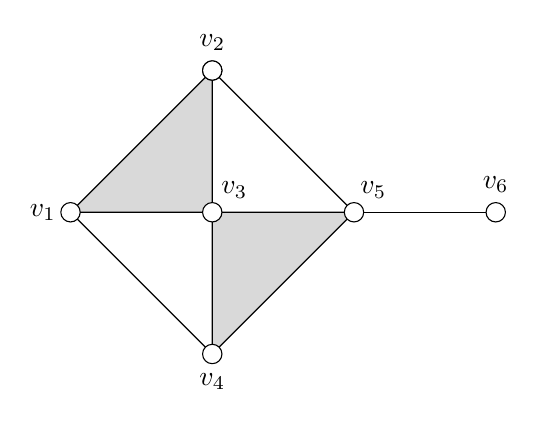
\begin{tikzpicture}[
      scale = .6,
      every node/.style={
        circle,
        draw=black,
        fill=white,
        inner sep=0pt,
        minimum size=7pt
      }
      ]

      \coordinate (v1) at (-3,0);
      \coordinate (v2) at (0,3);
      \coordinate (v3) at (0,0);
      \coordinate (v4) at (0,-3);
      \coordinate (v5) at (3,0);
      \coordinate (v6) at (6,0);

      \draw[fill=gray!30!white] (v1) -- (v2) -- (v3) -- (v1) -- cycle;
      \draw[fill=gray!30!white] (v3) -- (v4) -- (v5) -- (v3) -- cycle;

      \draw (v1) -- (v4);
      \draw (v2) -- (v5);
      \draw (v5) -- (v6);

      \node (wv1) at (v1) {};
      \node (wv2) at (v2) {};
      \node (vv2) at (v2) {};
      \node (vv3) at (v3) {};
      \node (vv4) at (v4) {};
      \node (vv5) at (v5) {};
      \node (vv6) at (v6) {};

      \node[draw=none, xshift=-1em] (wv1) at (v1) {$v_1$};
      \node[draw=none, yshift=1em] (wv2) at (v2) {$v_2$};
      \node[draw=none, xshift=.8em, yshift=.8em] (wv3) at (v3) {$v_3$};
      \node[draw=none, yshift=-1em] (wv4) at (v4) {$v_4$};
      \node[draw=none, xshift=.7em, yshift=.8em] (wv5) at (v5) {$v_5$};
      \node[draw=none, yshift=1em] (wv6) at (v6) {$v_6$};
    \end{tikzpicture}
    \caption{Simplicial complex $K$, straightened out}
  \end{figure}
  For the purposes of this problem, take angled brackets indicate span. We have
  \begin{enumerate}[label=(\roman*)]
  \item We calculate the $k=0$ case.
    \begin{enumerate}
    \item Elements of $\msf C_0(K)$ are formal linear combinations over the
      set $\set{v_1, v_2, \ldots, v_6}$. Then
      \[
        \msf C_0(K) = \ip[Big]{v_1, v_2, v_3, v_4, v_5, v_6}
      \]
      that is, collections of points in $\msf C_0(K)$.
    \item Let $\sigma_1, \ldots, \sigma_k \in \msf C_0(K).$ Then by definition,
      \begin{align*}
        \partial\pn{\sum_{i=1}^k \sigma_i}
        &= \sum_{i=1}^k \partial(\sigma_i)\\
        &= \sum_{i=1}^k 0 \\
        &= 0
      \end{align*}
      hence $\msf Z_n(K) = \msf C_n(K)$.
    \item A $\sigma \in \msf C_0(K)$ is an $n$-boundary if $\exists \tau \in
      \msf C_{1}(K)$ with $\partial(\tau) = \sigma$. Note, for any
      $1$-dimensional face $\set{v_iv_j} \in K$,
      \begin{align*}
        \partial(\set{v_iv_j})
        &= \set{v_i \widehat{v_j}} + \set{\widehat{v_i}v_j} \\
        &= \set{v_i} + \set{v_j} \\
        &= \delta_{ij}.
      \end{align*}
      Hence, any edge formed of a pair of two distinct vertices yields a
      nonempty boundary. We first count all edges:
      \begin{figure}[H]
        \centering
        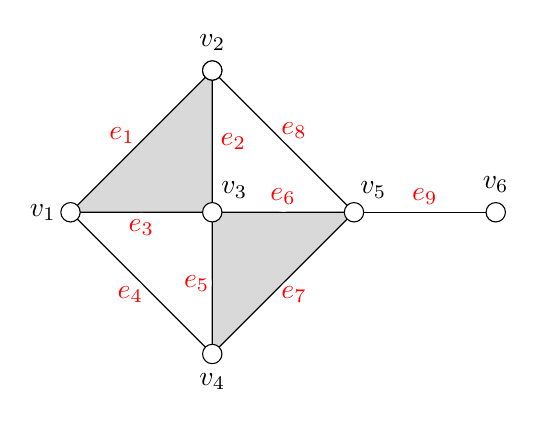
\begin{tikzpicture}[
          scale = .6,
          every node/.style={
            circle,
            draw=black,
            fill=white,
            inner sep=0pt,
            minimum size=7pt
          }
          ]

          \coordinate (v1) at (-3,0);
          \coordinate (v2) at (0,3);
          \coordinate (v3) at (0,0);
          \coordinate (v4) at (0,-3);
          \coordinate (v5) at (3,0);
          \coordinate (v6) at (6,0);

          \draw[fill=gray!30!white] (v1) -- (v2)
          % draw and label the edge between v1 and v2
          node[draw=none, midway, above left, xshift=-.3em, yshift=-.2em]
          {\color{red} $e_1$} -- (v3)
          % draw the edge between v2 and v3, and label it as well
          node[draw=none, midway, right, xshift=.2em] {\color{red} $e_2$}
          -- (v1)
          % draw the edge between v3 and v1, and label it as well
          node[draw=none, midway, below] {\color{red}$e_3$} -- cycle;

          \draw (v1) -- (v4) node[draw=none, midway, below left] {\color{red} $e_4$};

          \draw[fill=gray!30!white] (v3) -- (v4)
          % edge between v3 and and v4
          node[draw=none, midway, left] {\color{red} $e_5$} -- (v5)
          % edge
          node[draw=none, midway, below right] {\color{red}$e_7$} -- (v3)
          %
          node[draw=none, midway, above] {\color{red} $e_6$} -- cycle;


          \draw (v2) -- (v5) node[draw=none, midway, above right] {\color{red} $e_8$};
          \draw (v5) -- (v6) node[draw=none, midway, above] {\color{red} $e_9$};

          \node (wv1) at (v1) {};
          \node (wv2) at (v2) {};
          \node (vv2) at (v2) {};
          \node (vv3) at (v3) {};
          \node (vv4) at (v4) {};
          \node (vv5) at (v5) {};
          \node (vv6) at (v6) {};

          \node[draw=none, xshift=-1em] (wv1) at (v1) {$v_1$};
          \node[draw=none, yshift=1em] (wv2) at (v2) {$v_2$};
          \node[draw=none, xshift=.8em, yshift=.8em] (wv3) at (v3) {$v_3$};
          \node[draw=none, yshift=-1em] (wv4) at (v4) {$v_4$};
          \node[draw=none, xshift=.7em, yshift=.8em] (wv5) at (v5) {$v_5$};
          \node[draw=none, yshift=1em] (wv6) at (v6) {$v_6$};
        \end{tikzpicture}
        \caption{Simplicial complex $K$ with simple edges}
      \end{figure}
      Since $\msf B_0(K)$ is a subgroup of $\msf C_0(K)$, by closure under
      $+$, we see that any $v_i+v_j$ in $K$ such that there exists a path
      from $v_i$ to $v_j$ (when $K$ is considered a graph) is an element of
      $\msf B_0(K)$. In fact, we can say more:

      \textbf{Claim:} Since $K$ is connected as a graph, any even collection
      of vertices is in $\msf B_n(K)$.

      \textbf{Proof of Claim:} Suppose we have $\sigma = \set{v_{i_1}} +
      \set{v_{i_2}} + \cdots + \set{v_{i_{2k}}}$, where $k \in \NN$. Then
      for each $j = 1, \ldots, k$, let $\tau_j$ be a sum of edges representing
      a path from $v_{i_j}$ to $v_{i_{j+1}}$. For example, if $v_{i_j} =
      v_6$ and $v_{i_{j+1}} = v_2$, we could take the following approaches:
      \begin{figure}[H]
        \centering
        \begin{subfigure}{.49\linewidth}
          \centering
          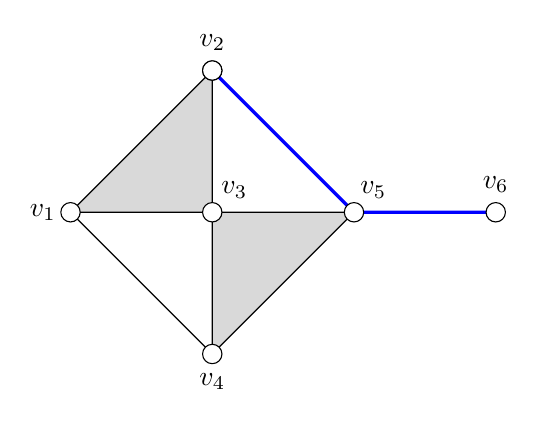
\begin{tikzpicture}[
            scale = .6,
            every node/.style={
              circle,
              draw=black,
              fill=white,
              inner sep=0pt,
              minimum size=7pt
            }
            ]

            \coordinate (v1) at (-3,0);
            \coordinate (v2) at (0,3);
            \coordinate (v3) at (0,0);
            \coordinate (v4) at (0,-3);
            \coordinate (v5) at (3,0);
            \coordinate (v6) at (6,0);

            \draw[fill=gray!30!white] (v1) -- (v2) -- (v3) -- (v1) -- cycle;
            \draw[fill=gray!30!white] (v3) -- (v4) -- (v5) -- (v3) -- cycle;

            \draw (v1) -- (v4);
            \draw (v2) -- (v5);
            \draw (v5) -- (v6);

            \draw[draw=blue, very thick] (v6) -- (v5) -- (v2);

            \node (wv1) at (v1) {};
            \node (wv2) at (v2) {};
            \node (vv2) at (v2) {};
            \node (vv3) at (v3) {};
            \node (vv4) at (v4) {};
            \node (vv5) at (v5) {};
            \node (vv6) at (v6) {};

            \node[draw=none, xshift=-1em] (wv1) at (v1) {$v_1$};
            \node[draw=none, yshift=1em] (wv2) at (v2) {$v_2$};
            \node[draw=none, xshift=.8em, yshift=.8em] (wv3) at (v3) {$v_3$};
            \node[draw=none, yshift=-1em] (wv4) at (v4) {$v_4$};
            \node[draw=none, xshift=.7em, yshift=.8em] (wv5) at (v5) {$v_5$};
            \node[draw=none, yshift=1em] (wv6) at (v6) {$v_6$};
          \end{tikzpicture}
        \end{subfigure}
        \begin{subfigure}{.49\linewidth}
          \centering
          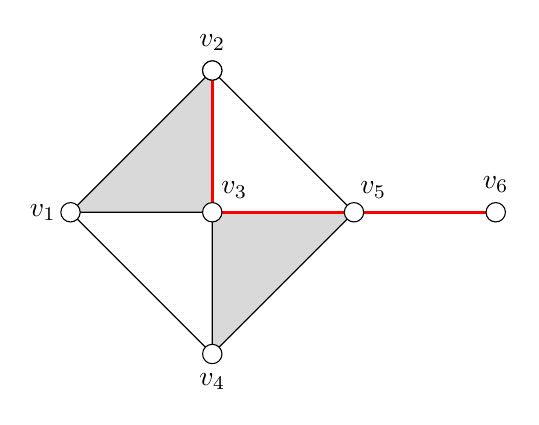
\begin{tikzpicture}[
            scale = .6,
            every node/.style={
              circle,
              draw=black,
              fill=white,
              inner sep=0pt,
              minimum size=7pt
            }
            ]

            \coordinate (v1) at (-3,0);
            \coordinate (v2) at (0,3);
            \coordinate (v3) at (0,0);
            \coordinate (v4) at (0,-3);
            \coordinate (v5) at (3,0);
            \coordinate (v6) at (6,0);

            \draw[fill=gray!30!white] (v1) -- (v2) -- (v3) -- (v1) -- cycle;
            \draw[fill=gray!30!white] (v3) -- (v4) -- (v5) -- (v3) -- cycle;

            \draw (v1) -- (v4);
            \draw (v2) -- (v5);
            \draw (v5) -- (v6);

            \draw[draw=red, very thick] (v6) -- (v5) -- (v3) -- (v2);

            \node (wv1) at (v1) {};
            \node (wv2) at (v2) {};
            \node (vv2) at (v2) {};
            \node (vv3) at (v3) {};
            \node (vv4) at (v4) {};
            \node (vv5) at (v5) {};
            \node (vv6) at (v6) {};

            \node[draw=none, xshift=-1em] (wv1) at (v1) {$v_1$};
            \node[draw=none, yshift=1em] (wv2) at (v2) {$v_2$};
            \node[draw=none, xshift=.8em, yshift=.8em] (wv3) at (v3) {$v_3$};
            \node[draw=none, yshift=-1em] (wv4) at (v4) {$v_4$};
            \node[draw=none, xshift=.7em, yshift=.8em] (wv5) at (v5) {$v_5$};
            \node[draw=none, yshift=1em] (wv6) at (v6) {$v_6$};
          \end{tikzpicture}
        \end{subfigure}
        \begin{subfigure}{.49\linewidth}
          \centering
          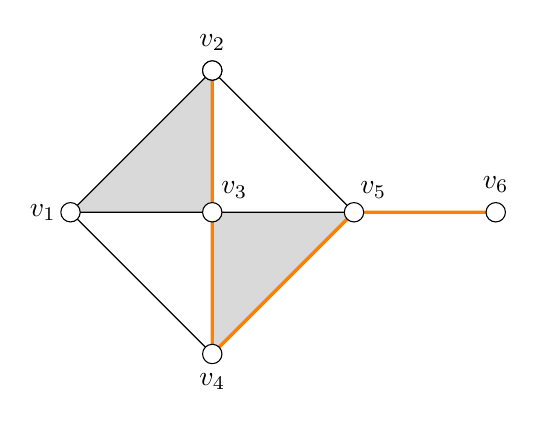
\begin{tikzpicture}[
            scale = .6,
            every node/.style={
              circle,
              draw=black,
              fill=white,
              inner sep=0pt,
              minimum size=7pt
            }
            ]

            \coordinate (v1) at (-3,0);
            \coordinate (v2) at (0,3);
            \coordinate (v3) at (0,0);
            \coordinate (v4) at (0,-3);
            \coordinate (v5) at (3,0);
            \coordinate (v6) at (6,0);

            \draw[fill=gray!30!white] (v1) -- (v2) -- (v3) -- (v1) -- cycle;
            \draw[fill=gray!30!white] (v3) -- (v4) -- (v5) -- (v3) -- cycle;

            \draw (v1) -- (v4);
            \draw (v2) -- (v5);
            \draw (v5) -- (v6);

            \draw[draw=orange, very thick] (v6) -- (v5) -- (v4) -- (v3)-- (v2);

            \node (wv1) at (v1) {};
            \node (wv2) at (v2) {};
            \node (vv2) at (v2) {};
            \node (vv3) at (v3) {};
            \node (vv4) at (v4) {};
            \node (vv5) at (v5) {};
            \node (vv6) at (v6) {};

            \node[draw=none, xshift=-1em] (wv1) at (v1) {$v_1$};
            \node[draw=none, yshift=1em] (wv2) at (v2) {$v_2$};
            \node[draw=none, xshift=.8em, yshift=.8em] (wv3) at (v3) {$v_3$};
            \node[draw=none, yshift=-1em] (wv4) at (v4) {$v_4$};
            \node[draw=none, xshift=.7em, yshift=.8em] (wv5) at (v5) {$v_5$};
            \node[draw=none, yshift=1em] (wv6) at (v6) {$v_6$};
          \end{tikzpicture}
        \end{subfigure}
        \begin{subfigure}{.49\linewidth}
          \centering
          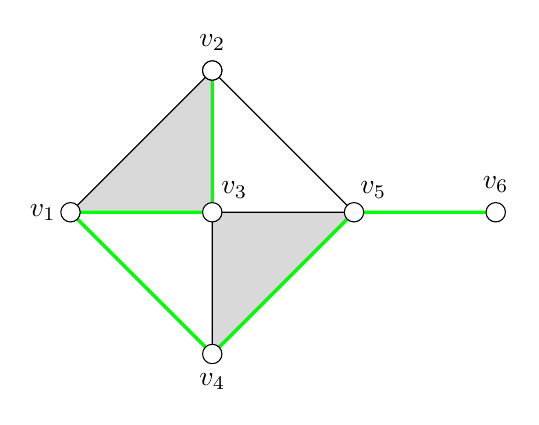
\begin{tikzpicture}[
            scale = .6,
            every node/.style={
              circle,
              draw=black,
              fill=white,
              inner sep=0pt,
              minimum size=7pt
            }
            ]

            \coordinate (v1) at (-3,0);
            \coordinate (v2) at (0,3);
            \coordinate (v3) at (0,0);
            \coordinate (v4) at (0,-3);
            \coordinate (v5) at (3,0);
            \coordinate (v6) at (6,0);

            \draw[fill=gray!30!white] (v1) -- (v2) -- (v3) -- (v1) -- cycle;
            \draw[fill=gray!30!white] (v3) -- (v4) -- (v5) -- (v3) -- cycle;

            \draw (v1) -- (v4);
            \draw (v2) -- (v5);
            \draw (v5) -- (v6);

            \draw[draw=green, very thick] (v6) -- (v5) -- (v4) -- (v1) -- (v3) -- (v2);

            \node (wv1) at (v1) {};
            \node (wv2) at (v2) {};
            \node (vv2) at (v2) {};
            \node (vv3) at (v3) {};
            \node (vv4) at (v4) {};
            \node (vv5) at (v5) {};
            \node (vv6) at (v6) {};

            \node[draw=none, xshift=-1em] (wv1) at (v1) {$v_1$};
            \node[draw=none, yshift=1em] (wv2) at (v2) {$v_2$};
            \node[draw=none, xshift=.8em, yshift=.8em] (wv3) at (v3) {$v_3$};
            \node[draw=none, yshift=-1em] (wv4) at (v4) {$v_4$};
            \node[draw=none, xshift=.7em, yshift=.8em] (wv5) at (v5) {$v_5$};
            \node[draw=none, yshift=1em] (wv6) at (v6) {$v_6$};
          \end{tikzpicture}
        \end{subfigure}
      \end{figure}\clearpage
      \begin{figure}[H]\ContinuedFloat
        \begin{subfigure}{.49\linewidth}
          \centering
          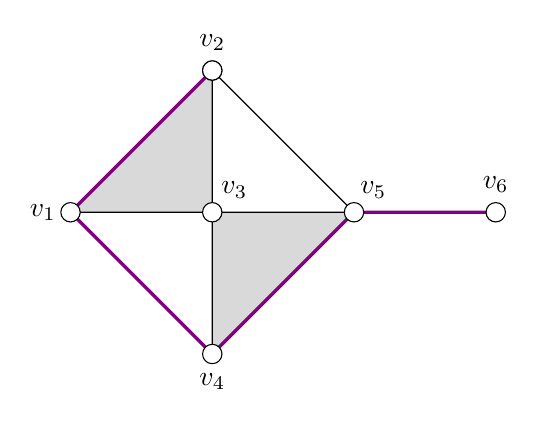
\begin{tikzpicture}[
            scale = .6,
            every node/.style={
              circle,
              draw=black,
              fill=white,
              inner sep=0pt,
              minimum size=7pt
            }
            ]

            \coordinate (v1) at (-3,0);
            \coordinate (v2) at (0,3);
            \coordinate (v3) at (0,0);
            \coordinate (v4) at (0,-3);
            \coordinate (v5) at (3,0);
            \coordinate (v6) at (6,0);

            \draw[fill=gray!30!white] (v1) -- (v2) -- (v3) -- (v1) -- cycle;
            \draw[fill=gray!30!white] (v3) -- (v4) -- (v5) -- (v3) -- cycle;

            \draw (v1) -- (v4);
            \draw (v2) -- (v5);
            \draw (v5) -- (v6);

            \draw[draw=violet, very thick] (v6) -- (v5) -- (v4) -- (v1)-- (v2);

            \node (wv1) at (v1) {};
            \node (wv2) at (v2) {};
            \node (vv2) at (v2) {};
            \node (vv3) at (v3) {};
            \node (vv4) at (v4) {};
            \node (vv5) at (v5) {};
            \node (vv6) at (v6) {};

            \node[draw=none, xshift=-1em] (wv1) at (v1) {$v_1$};
            \node[draw=none, yshift=1em] (wv2) at (v2) {$v_2$};
            \node[draw=none, xshift=.8em, yshift=.8em] (wv3) at (v3) {$v_3$};
            \node[draw=none, yshift=-1em] (wv4) at (v4) {$v_4$};
            \node[draw=none, xshift=.7em, yshift=.8em] (wv5) at (v5) {$v_5$};
            \node[draw=none, yshift=1em] (wv6) at (v6) {$v_6$};
          \end{tikzpicture}
        \end{subfigure}
        \begin{subfigure}{.49\linewidth}
          \centering
          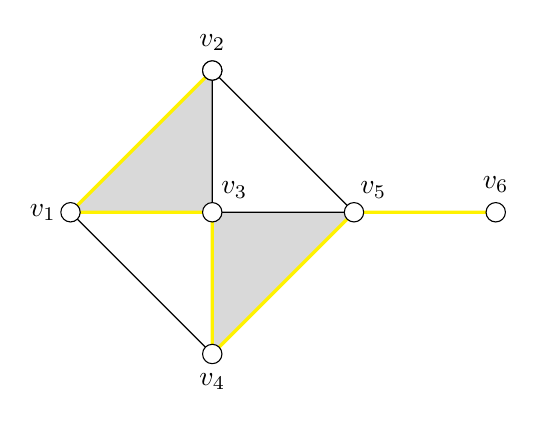
\begin{tikzpicture}[
            scale = .6,
            every node/.style={
              circle,
              draw=black,
              fill=white,
              inner sep=0pt,
              minimum size=7pt
            }
            ]

            \coordinate (v1) at (-3,0);
            \coordinate (v2) at (0,3);
            \coordinate (v3) at (0,0);
            \coordinate (v4) at (0,-3);
            \coordinate (v5) at (3,0);
            \coordinate (v6) at (6,0);

            \draw[fill=gray!30!white] (v1) -- (v2) -- (v3) -- (v1) -- cycle;
            \draw[fill=gray!30!white] (v3) -- (v4) -- (v5) -- (v3) -- cycle;

            \draw (v1) -- (v4);
            \draw (v2) -- (v5);
            \draw (v5) -- (v6);

            \draw[draw=yellow, very thick] (v6) -- (v5) -- (v4) -- (v3) -- (v1) -- (v2);

            \node (wv1) at (v1) {};
            \node (wv2) at (v2) {};
            \node (vv2) at (v2) {};
            \node (vv3) at (v3) {};
            \node (vv4) at (v4) {};
            \node (vv5) at (v5) {};
            \node (vv6) at (v6) {};

            \node[draw=none, xshift=-1em] (wv1) at (v1) {$v_1$};
            \node[draw=none, yshift=1em] (wv2) at (v2) {$v_2$};
            \node[draw=none, xshift=.8em, yshift=.8em] (wv3) at (v3) {$v_3$};
            \node[draw=none, yshift=-1em] (wv4) at (v4) {$v_4$};
            \node[draw=none, xshift=.7em, yshift=.8em] (wv5) at (v5) {$v_5$};
            \node[draw=none, yshift=1em] (wv6) at (v6) {$v_6$};
          \end{tikzpicture}
        \end{subfigure}
        \caption{Some paths from $v_6$ to $v_2$}
      \end{figure}
      among others. Taking the sum of the constituent edges in each path
      yields a sum of $1$-simplices with boundary $v_6,
      v_2$.\footnote{Justification: note that the coefficient on any given
        vertex when we apply $\partial$ is the degree of the vertex in our
        path. Hence, only the initial and terminal vertex don't get mapped
        to $0$.}
    \item Since $\msf B_n(K)$ is the group of all collections of even
      vertices in $\msf C_n(K)$, we have $\msf H_n(K) = \msf C_n(K)/\msf
      B_n(K) \cong \zmod{2}$.
    \end{enumerate}
  \item Now, we calculate the $k=1$ case.
    \begin{enumerate}
    \item Elements of $\msf C_1(K)$ are collections of linear combinations
      of the edges
      \[
        \msf C_1(K) = \ip{e_1, e_2, e_3, e_4, e_5, e_6, e_7, e_8, e_9}
      \]
    \item Elements of $\msf Z_1(K)$ are collections of edges such that
      each vertex contained in an edge in the collection has even degree.
      This corresponds to cyclic subgraphs of $K$ (as well as the empty
      cycle), e.g.:
      \begin{figure}[H]
        \centering
        \begin{subfigure}{.49\linewidth}
          \centering
          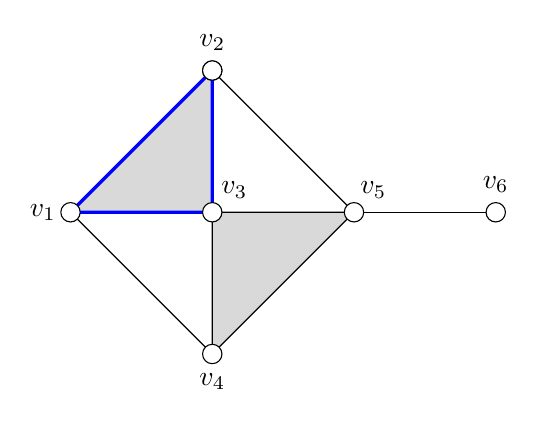
\begin{tikzpicture}[
            scale = .6,
            every node/.style={
              circle,
              draw=black,
              fill=white,
              inner sep=0pt,
              minimum size=7pt
            }
            ]

            \coordinate (v1) at (-3,0);
            \coordinate (v2) at (0,3);
            \coordinate (v3) at (0,0);
            \coordinate (v4) at (0,-3);
            \coordinate (v5) at (3,0);
            \coordinate (v6) at (6,0);

            \draw[fill=gray!30!white] (v1) -- (v2) -- (v3) -- (v1) -- cycle;
            \draw[fill=gray!30!white] (v3) -- (v4) -- (v5) -- (v3) -- cycle;

            \draw (v1) -- (v4);
            \draw (v2) -- (v5);
            \draw (v5) -- (v6);

            \draw[draw=blue, very thick] (v1) -- (v2) -- (v3) -- cycle;

            \node (wv1) at (v1) {};
            \node (wv2) at (v2) {};
            \node (vv2) at (v2) {};
            \node (vv3) at (v3) {};
            \node (vv4) at (v4) {};
            \node (vv5) at (v5) {};
            \node (vv6) at (v6) {};

            \node[draw=none, xshift=-1em] (wv1) at (v1) {$v_1$};
            \node[draw=none, yshift=1em] (wv2) at (v2) {$v_2$};
            \node[draw=none, xshift=.8em, yshift=.8em] (wv3) at (v3) {$v_3$};
            \node[draw=none, yshift=-1em] (wv4) at (v4) {$v_4$};
            \node[draw=none, xshift=.7em, yshift=.8em] (wv5) at (v5) {$v_5$};
            \node[draw=none, yshift=1em] (wv6) at (v6) {$v_6$};
          \end{tikzpicture}
        \end{subfigure}
        \begin{subfigure}{.49\linewidth}
          \centering
          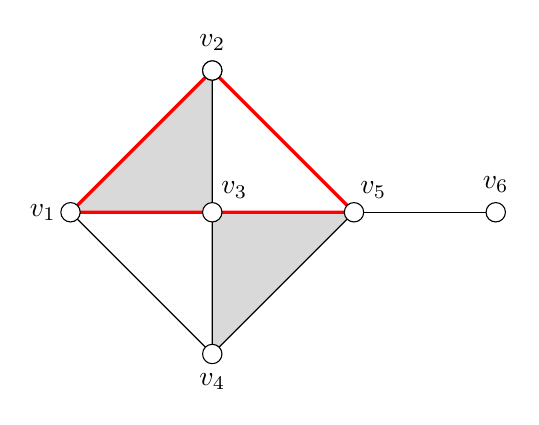
\begin{tikzpicture}[
            scale = .6,
            every node/.style={
              circle,
              draw=black,
              fill=white,
              inner sep=0pt,
              minimum size=7pt
            }
            ]

            \coordinate (v1) at (-3,0);
            \coordinate (v2) at (0,3);
            \coordinate (v3) at (0,0);
            \coordinate (v4) at (0,-3);
            \coordinate (v5) at (3,0);
            \coordinate (v6) at (6,0);

            \draw[fill=gray!30!white] (v1) -- (v2) -- (v3) -- (v1) -- cycle;
            \draw[fill=gray!30!white] (v3) -- (v4) -- (v5) -- (v3) -- cycle;

            \draw (v1) -- (v4);
            \draw (v2) -- (v5);
            \draw (v5) -- (v6);

            \draw[draw=red, very thick] (v1) -- (v2) -- (v5) -- (v3) -- (v1);

            \node (wv1) at (v1) {};
            \node (wv2) at (v2) {};
            \node (vv2) at (v2) {};
            \node (vv3) at (v3) {};
            \node (vv4) at (v4) {};
            \node (vv5) at (v5) {};
            \node (vv6) at (v6) {};

            \node[draw=none, xshift=-1em] (wv1) at (v1) {$v_1$};
            \node[draw=none, yshift=1em] (wv2) at (v2) {$v_2$};
            \node[draw=none, xshift=.8em, yshift=.8em] (wv3) at (v3) {$v_3$};
            \node[draw=none, yshift=-1em] (wv4) at (v4) {$v_4$};
            \node[draw=none, xshift=.7em, yshift=.8em] (wv5) at (v5) {$v_5$};
            \node[draw=none, yshift=1em] (wv6) at (v6) {$v_6$};
          \end{tikzpicture}
        \end{subfigure}
      \end{figure}
      \clearpage
      \begin{figure}[H]\ContinuedFloat
        \begin{subfigure}{.49\linewidth}
          \centering
          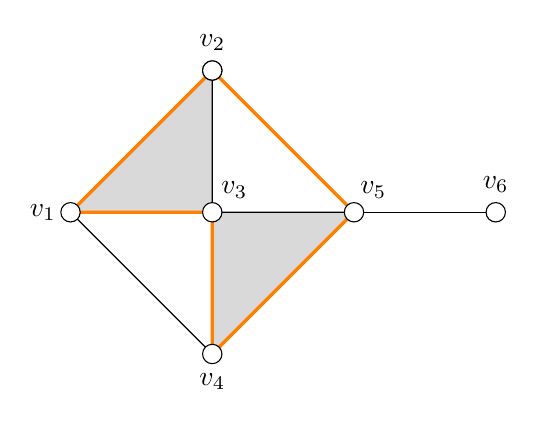
\begin{tikzpicture}[
            scale = .6,
            every node/.style={
              circle,
              draw=black,
              fill=white,
              inner sep=0pt,
              minimum size=7pt
            }
            ]

            \coordinate (v1) at (-3,0);
            \coordinate (v2) at (0,3);
            \coordinate (v3) at (0,0);
            \coordinate (v4) at (0,-3);
            \coordinate (v5) at (3,0);
            \coordinate (v6) at (6,0);

            \draw[fill=gray!30!white] (v1) -- (v2) -- (v3) -- (v1) -- cycle;
            \draw[fill=gray!30!white] (v3) -- (v4) -- (v5) -- (v3) -- cycle;

            \draw (v1) -- (v4);
            \draw (v2) -- (v5);
            \draw (v5) -- (v6);

            \draw[draw=orange, very thick] (v1) -- (v2) -- (v5) -- (v4)-- (v3) -- cycle;

            \node (wv1) at (v1) {};
            \node (wv2) at (v2) {};
            \node (vv2) at (v2) {};
            \node (vv3) at (v3) {};
            \node (vv4) at (v4) {};
            \node (vv5) at (v5) {};
            \node (vv6) at (v6) {};

            \node[draw=none, xshift=-1em] (wv1) at (v1) {$v_1$};
            \node[draw=none, yshift=1em] (wv2) at (v2) {$v_2$};
            \node[draw=none, xshift=.8em, yshift=.8em] (wv3) at (v3) {$v_3$};
            \node[draw=none, yshift=-1em] (wv4) at (v4) {$v_4$};
            \node[draw=none, xshift=.7em, yshift=.8em] (wv5) at (v5) {$v_5$};
            \node[draw=none, yshift=1em] (wv6) at (v6) {$v_6$};
          \end{tikzpicture}
        \end{subfigure}
        \begin{subfigure}{.49\linewidth}
          \centering
          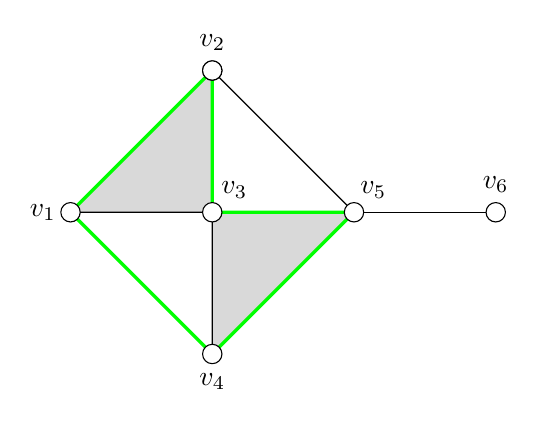
\begin{tikzpicture}[
            scale = .6,
            every node/.style={
              circle,
              draw=black,
              fill=white,
              inner sep=0pt,
              minimum size=7pt
            }
            ]

            \coordinate (v1) at (-3,0);
            \coordinate (v2) at (0,3);
            \coordinate (v3) at (0,0);
            \coordinate (v4) at (0,-3);
            \coordinate (v5) at (3,0);
            \coordinate (v6) at (6,0);

            \draw[fill=gray!30!white] (v1) -- (v2) -- (v3) -- (v1) -- cycle;
            \draw[fill=gray!30!white] (v3) -- (v4) -- (v5) -- (v3) -- cycle;

            \draw (v1) -- (v4);
            \draw (v2) -- (v5);
            \draw (v5) -- (v6);

            \draw[draw=green, very thick] (v1) -- (v2) -- (v3) -- (v5) -- (v4) -- cycle;

            \node (wv1) at (v1) {};
            \node (wv2) at (v2) {};
            \node (vv2) at (v2) {};
            \node (vv3) at (v3) {};
            \node (vv4) at (v4) {};
            \node (vv5) at (v5) {};
            \node (vv6) at (v6) {};

            \node[draw=none, xshift=-1em] (wv1) at (v1) {$v_1$};
            \node[draw=none, yshift=1em] (wv2) at (v2) {$v_2$};
            \node[draw=none, xshift=.8em, yshift=.8em] (wv3) at (v3) {$v_3$};
            \node[draw=none, yshift=-1em] (wv4) at (v4) {$v_4$};
            \node[draw=none, xshift=.7em, yshift=.8em] (wv5) at (v5) {$v_5$};
            \node[draw=none, yshift=1em] (wv6) at (v6) {$v_6$};
          \end{tikzpicture}
        \end{subfigure}
        \begin{subfigure}{.49\linewidth}
          \centering
          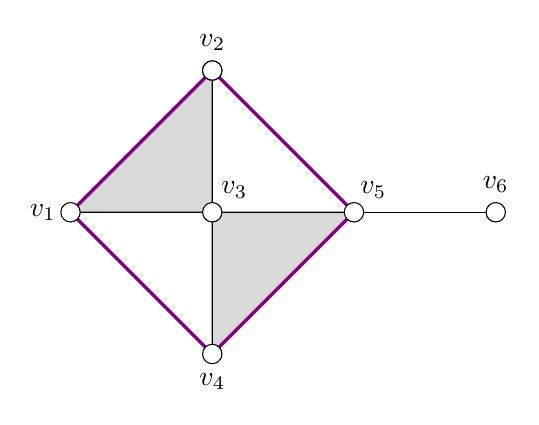
\begin{tikzpicture}[
            scale = .6,
            every node/.style={
              circle,
              draw=black,
              fill=white,
              inner sep=0pt,
              minimum size=7pt
            }
            ]

            \coordinate (v1) at (-3,0);
            \coordinate (v2) at (0,3);
            \coordinate (v3) at (0,0);
            \coordinate (v4) at (0,-3);
            \coordinate (v5) at (3,0);
            \coordinate (v6) at (6,0);

            \draw[fill=gray!30!white] (v1) -- (v2) -- (v3) -- (v1) -- cycle;
            \draw[fill=gray!30!white] (v3) -- (v4) -- (v5) -- (v3) -- cycle;

            \draw (v1) -- (v4);
            \draw (v2) -- (v5);
            \draw (v5) -- (v6);

            \draw[draw=violet, very thick] (v1) -- (v2) -- (v5) -- (v4) -- cycle;

            \node (wv1) at (v1) {};
            \node (wv2) at (v2) {};
            \node (vv2) at (v2) {};
            \node (vv3) at (v3) {};
            \node (vv4) at (v4) {};
            \node (vv5) at (v5) {};
            \node (vv6) at (v6) {};

            \node[draw=none, xshift=-1em] (wv1) at (v1) {$v_1$};
            \node[draw=none, yshift=1em] (wv2) at (v2) {$v_2$};
            \node[draw=none, xshift=.8em, yshift=.8em] (wv3) at (v3) {$v_3$};
            \node[draw=none, yshift=-1em] (wv4) at (v4) {$v_4$};
            \node[draw=none, xshift=.7em, yshift=.8em] (wv5) at (v5) {$v_5$};
            \node[draw=none, yshift=1em] (wv6) at (v6) {$v_6$};
          \end{tikzpicture}
        \end{subfigure}
        \begin{subfigure}{.49\linewidth}
          \centering
          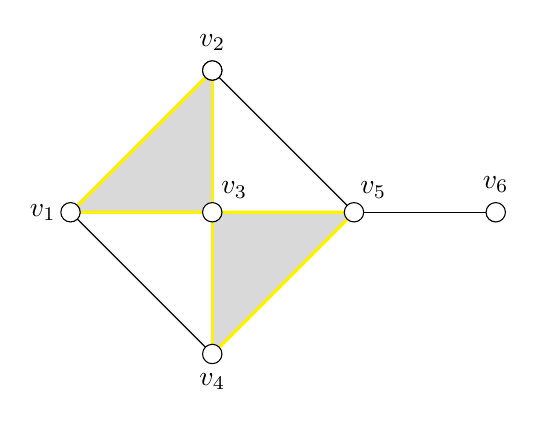
\begin{tikzpicture}[
            scale = .6,
            every node/.style={
              circle,
              draw=black,
              fill=white,
              inner sep=0pt,
              minimum size=7pt
            }
            ]

            \coordinate (v1) at (-3,0);
            \coordinate (v2) at (0,3);
            \coordinate (v3) at (0,0);
            \coordinate (v4) at (0,-3);
            \coordinate (v5) at (3,0);
            \coordinate (v6) at (6,0);

            \draw[fill=gray!30!white] (v1) -- (v2) -- (v3) -- (v1) -- cycle;
            \draw[fill=gray!30!white] (v3) -- (v4) -- (v5) -- (v3) -- cycle;

            \draw (v1) -- (v4);
            \draw (v2) -- (v5);
            \draw (v5) -- (v6);

            \draw[draw=yellow, very thick] (v1) -- (v2) -- (v3) -- cycle;
            \draw[draw=yellow, very thick] (v3) -- (v4) -- (v5) -- cycle;

            \node (wv1) at (v1) {};
            \node (wv2) at (v2) {};
            \node (vv2) at (v2) {};
            \node (vv3) at (v3) {};
            \node (vv4) at (v4) {};
            \node (vv5) at (v5) {};
            \node (vv6) at (v6) {};

            \node[draw=none, xshift=-1em] (wv1) at (v1) {$v_1$};
            \node[draw=none, yshift=1em] (wv2) at (v2) {$v_2$};
            \node[draw=none, xshift=.8em, yshift=.8em] (wv3) at (v3) {$v_3$};
            \node[draw=none, yshift=-1em] (wv4) at (v4) {$v_4$};
            \node[draw=none, xshift=.7em, yshift=.8em] (wv5) at (v5) {$v_5$};
            \node[draw=none, yshift=1em] (wv6) at (v6) {$v_6$};
          \end{tikzpicture}
        \end{subfigure}
        \caption{Some cycles in $K$}
      \end{figure}
    \item First, consider the following diagram:
      \begin{figure}[H]
        \centering
        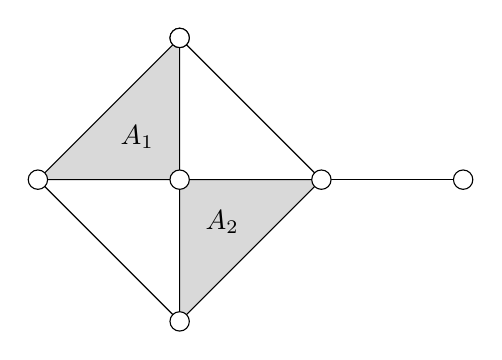
\begin{tikzpicture}[
          scale = .6,
          every node/.style={
            circle,
            draw=black,
            fill=white,
            inner sep=0pt,
            minimum size=7pt
          }
          ]

          \coordinate (v1) at (-3,0);
          \coordinate (v2) at (0,3);
          \coordinate (v3) at (0,0);
          \coordinate (v4) at (0,-3);
          \coordinate (v5) at (3,0);
          \coordinate (v6) at (6,0);

          \draw[fill=gray!30!white] (v1) -- (v2) -- (v3) -- (v1) -- cycle;

          \draw (v1) -- (v4);

          \draw[fill=gray!30!white] (v3) -- (v4) -- (v5) -- (v3) -- cycle;


          \draw (v2) -- (v5) ;
          \draw (v5) -- (v6) ;

          \node (wv1) at (v1) {};
          \node (wv2) at (v2) {};
          \node (vv2) at (v2) {};
          \node (vv3) at (v3) {};
          \node (vv4) at (v4) {};
          \node (vv5) at (v5) {};
          \node (vv6) at (v6) {};

          \node[draw=none,fill=none] (a1) at (-.9,.9) {$A_1$};
          \node[draw=none,fill=none] (a1) at (.9,-.9) {$A_2$};
        \end{tikzpicture}
        \caption{Two $n=2$ simplices}
      \end{figure}
      $\mb 0_1$ bounds $\mb 0_2$. Since $\partial(A_1) \cap \partial(A_2) =
      \varnothing$, then the other two cycles in $\msf B_1(K)$ are just
      $\partial(A_1)$ and $\partial(A_2)$, respectively.
    \item $\msf H_1(K) \cong \zmod{2} \times \zmod{2}$ (equivalence classes
      have representative elements $\mb 0, \partial(A_1), \partial(A_2),
      \partial(A_1) + \partial(A_2)$)
    \end{enumerate}
  \item For $k=2$, we have
    \begin{enumerate}
    \item $\msf C_2(K) \cong \zmod{2} \times \zmod{2}$
    \item $\msf Z_2(K) \cong \mb 0$
    \item $\msf B_2(K) \cong \mb 0$
    \item And hence $\msf H_2(K) \cong \mb 0$.
    \end{enumerate}
  \end{enumerate}
\end{solution}
\begin{problem}[16.7]
  If $K$ is a one-point space, $\msf H_n(K) \cong 0$ for $n \geq 0$, and $\msf
  H_0(K) \cong \zmod{2}$.
\end{problem}
\begin{solution}
  For $n > 0$, $\msf C_n(K)$ is the trivial group. Since $\msf Z_n(K) \leq \msf
  C_n(K)$, we thus have $\msf Z_n(K) \cong 0$, and so $\msf H_n(K) \cong 0$.

  For the $n = 0$, note that $\msf Z_0(K) = \msf C_0(K) \cong \zmod{2}$ (every
  point is definitionally a 0-cycle). Since $K$ contains no 1-simplices, $\msf
  B_0(K) = \mb 0$, hence $\msf H_0(K) \cong \zmod{2}$.
\end{solution}
\begin{definition}[Simplicially connected]
  Let $K$ be a simplicial complex. Then we call $K$ \emph{simplicially
    connected} iff for all pairs of 0-simplices $v_0, v_n \in K$, there exists a
  sequence of 0-simplices $\set{v_i}_{i\in [n]}$ such that for all $i \in [n]$
  (with $i \neq n$), $\set{v_iv_{i+1}}$ is a 1-simplex in $K$. Note, this
  corresponds exactly to $K$ being connected as a graph, where the 0-simplices
  represent vertices, and the 1-simplices represent edges.
\end{definition}
\begin{problem}[16.8]
  If $K$ is simplicially connected, then $\msf H_0(K) \cong \zmod{2}$. If $K$
  has $r$ simplicially connected components, then
  \[
    \msf H_0(K)\cong \prod_{i=1}^r \zmod{2}
  \]
\end{problem}
\begin{solution}
  \begin{enumerate}
  \item Suppose $K$ is simplicially connected. We want to show $\msf H_0(K)
    \cong \zmod{2}$. First, observe that $\msf Z_0(K) \cong \msf C_0(K)$
    (every 0 simplex has trivial boundary). By properties of module
    homomorphisms, for all $\sigma \in \msf B_0(K)$, $\sigma$ is a basis
    element of $\msf B_0(K)$ iff $\exists \tau \in \msf C_1(K)$ such that
    $\tau$ is a basis element of $\msf C_1(K)$, and $\partial_1(\tau) =
    \sigma$. Thus, $\msf B_0(K)$ is spanned by $\set{\set{\set{v_i} +
        \set{v_j}} \MID \set{v_iv_j} \in K}$. It follows that $\msf B_0(K)$
    contains exactly those elements of $\msf C_0(K)$ with an even number of
    vertices.\footnote{Since $\msf B_0(K)$ is generated by pairs.}

    It follows that $\msf H_0(K) = \msf Z_0(K)/\msf B_0(K) \cong \zmod{2}$
    (any $0$-chain has either an even or odd number of vertices).
  \item This follows by applying the above argument to each of the connected
    components.
  \end{enumerate}
\end{solution}
\begin{problem}[16.9]
  Let $K$ be a triangulation of a $3$-dimensional ball that consists of a
  3-simplex together with its faces. Compute $\msf H_n(K)$ for each $n$.
\end{problem}
\begin{solution}
  \begin{figure}[H]
    \centering
    \begin{subfigure}{\linewidth}
      \centering
      \tdplotsetmaincoords{70}{80}
      \begin{tikzpicture}[tdplot_main_coords,scale=2]
        \path
        coordinate (A) at (0,0,0)
        coordinate (B) at (2,0,0)
        coordinate (C) at (1,1.732,0)
        coordinate (D) at (1,.577,1.733);

        \draw [dashed] (A)--(C);
        \fill [opacity=.5, red!30!white] (A) -- (B) -- (C) -- cycle;
        \fill [opacity=.5, blue!30!white] (D) -- (B) -- (A) -- cycle;
        \fill [opacity=.5, green!30!white] (D) -- (A) -- (C) -- cycle;
        \draw[thick] (A) -- (B) (A) -- (D);
        \draw[thick, fill opacity=.5, fill=orange!30!white] (D) -- (B) -- (C) -- cycle;

        \node (V) at (1,.577,.433) {\LARGE $V_1$};

        \foreach \v/\position in {A/left,B/below,C/right,D/above} {
          \draw[fill=black] (\v) circle (0.5pt) node [\position=0.2mm] {$\v$};
        }
      \end{tikzpicture}
    \end{subfigure}\\\vspace{1cm}
    \begin{subfigure}{.24\linewidth}
      \centering
      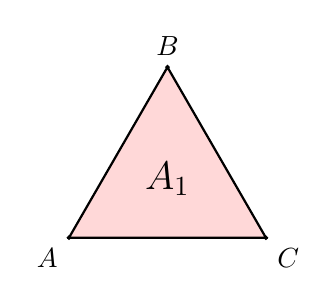
\begin{tikzpicture}[scale=1.25]
        \path
        coordinate (A) at (0,0)
        coordinate (C) at (2,0)
        coordinate (B) at (1,1.732);

        \draw[thick, fill opacity=.5, fill=red!30!white] (A) -- (B) -- (C) -- cycle;

        \node (A1) at (1,.6) {\Large $A_1$};

        \foreach \v/\position in {A/below left, C/below right, B/above} {
          \draw[fill=black] (\v) circle (0.5pt) node [\position=0.2mm] {$\v$};
        }
      \end{tikzpicture}
    \end{subfigure}
    \begin{subfigure}{.24\linewidth}
      \centering
      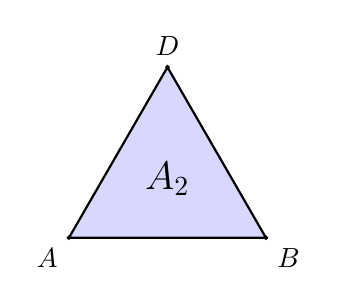
\begin{tikzpicture}[scale=1.25]
        \path
        coordinate (A) at (0,0)
        coordinate (B) at (2,0)
        coordinate (D) at (1,1.732);

        \draw[thick, fill opacity=.5, fill=blue!30!white] (D) -- (B) -- (A) -- cycle;

        \node (A2) at (1,.6) {\Large $A_2$};

        \foreach \v/\position in {A/below left, B/below right, D/above} {
          \draw[fill=black] (\v) circle (0.5pt) node [\position=0.2mm] {$\v$};
        }
      \end{tikzpicture}
    \end{subfigure}
    \begin{subfigure}{.24\linewidth}
      \centering
      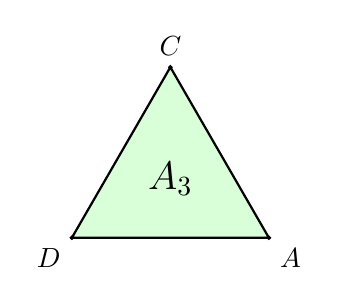
\begin{tikzpicture}[scale=1.25]
        \path
        coordinate (D) at (0,0)
        coordinate (A) at (2,0)
        coordinate (C) at (1,1.732);

        \draw[thick, fill opacity=.5, fill=green!30!white] (D) -- (A) -- (C) -- cycle;

        \node (A3) at (1,.6) {\Large $A_3$};

        \foreach \v/\position in {D/below left, A/below right, C/above} {
          \draw[fill=black] (\v) circle (0.5pt) node [\position=0.2mm] {$\v$};
        }
      \end{tikzpicture}
    \end{subfigure}
    \begin{subfigure}{.24\linewidth}
      \centering
      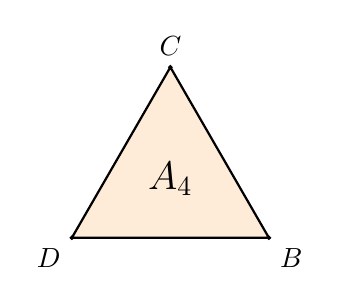
\begin{tikzpicture}[scale=1.25]
        \path
        coordinate (D) at (0,0)
        coordinate (B) at (2,0)
        coordinate (C) at (1,1.732);

        \draw[thick, fill opacity=.5, fill=orange!30!white] (D) -- (B) -- (C) -- cycle;

        \node (A4) at (1,.6) {\Large $A_4$};

        \foreach \v/\position in {D/below left, B/below right, C/above} {
          \draw[fill=black] (\v) circle (0.5pt) node [\position=0.2mm] {$\v$};
        }
      \end{tikzpicture}
    \end{subfigure}\\\vspace{1cm}
    \tikzset{
      brace/.style={
        thick,
        decoration={brace, mirror, raise=1pt, amplitude=6pt},
        decorate
      },
      blabel/.style={
        right, pos=.5, xshift=7pt, yshift=-2pt
      }
    }
    \begin{subfigure}{.161\linewidth}
      \centering
      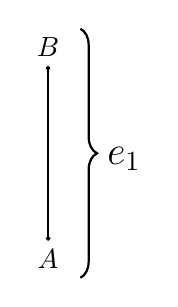
\begin{tikzpicture}[scale=1.25]
        \def\firstcoord{A}
        \def\secondcoord{B}
        \path coordinate (\firstcoord) at (0,0) coordinate (\secondcoord) at (0,1.73);
        \draw[thick] (\firstcoord) -- (\secondcoord);

        \draw[brace] (.3,-.4) -- node[blabel] {\Large $e_1$} (.3,2.13);

        \foreach \v/\position in {\firstcoord/below, \secondcoord/above} {
          \draw[fill=black] (\v) circle (0.5pt) node [\position=0.2mm] {$\v$};
        }
      \end{tikzpicture}
    \end{subfigure}
    \begin{subfigure}{.161\linewidth}
      \centering
      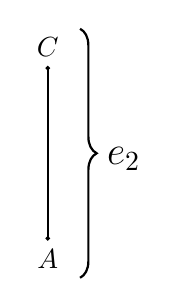
\begin{tikzpicture}[scale=1.25]
        \def\firstcoord{A}
        \def\secondcoord{C}
        \path coordinate (\firstcoord) at (0,0) coordinate (\secondcoord) at (0,1.73);
        \draw[thick] (\firstcoord) -- (\secondcoord);

        \draw[brace] (.3,-.4) -- node[blabel] {\Large $e_2$} (.3,2.13);

        \foreach \v/\position in {\firstcoord/below, \secondcoord/above} {
          \draw[fill=black] (\v) circle (0.5pt) node [\position=0.2mm] {$\v$};
        }
      \end{tikzpicture}
    \end{subfigure}
    \begin{subfigure}{.161\linewidth}
      \centering
      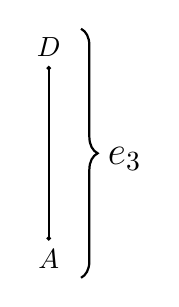
\begin{tikzpicture}[scale=1.25]
        \def\firstcoord{A}
        \def\secondcoord{D}
        \path coordinate (\firstcoord) at (0,0) coordinate (\secondcoord) at (0,1.73);
        \draw[thick] (\firstcoord) -- (\secondcoord);

        \draw[brace] (.3,-.4) -- node[blabel] {\Large $e_3$} (.3,2.13);

        \foreach \v/\position in {\firstcoord/below, \secondcoord/above} {
          \draw[fill=black] (\v) circle (0.5pt) node [\position=0.2mm] {$\v$};
        }
      \end{tikzpicture}
    \end{subfigure}
    \begin{subfigure}{.161\linewidth}
      \centering
      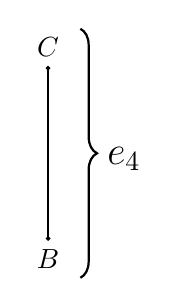
\begin{tikzpicture}[scale=1.25]
        \def\firstcoord{B}
        \def\secondcoord{C}
        \path coordinate (\firstcoord) at (0,0) coordinate (\secondcoord) at (0,1.73);
        \draw[thick] (\firstcoord) -- (\secondcoord);

        \draw[brace] (.3,-.4) -- node[blabel] {\Large $e_4$} (.3,2.13);

        \foreach \v/\position in {\firstcoord/below, \secondcoord/above} {
          \draw[fill=black] (\v) circle (0.5pt) node [\position=0.2mm] {$\v$};
        }
      \end{tikzpicture}
    \end{subfigure}
    \begin{subfigure}{.161\linewidth}
      \centering
      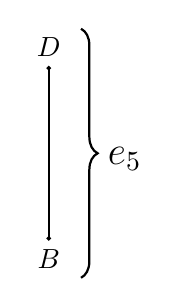
\begin{tikzpicture}[scale=1.25]
        \def\firstcoord{B}
        \def\secondcoord{D}
        \path coordinate (\firstcoord) at (0,0) coordinate (\secondcoord) at (0,1.73);
        \draw[thick] (\firstcoord) -- (\secondcoord);

        \draw[brace] (.3,-.4) -- node[blabel] {\Large $e_5$} (.3,2.13);

        \foreach \v/\position in {\firstcoord/below, \secondcoord/above} {
          \draw[fill=black] (\v) circle (0.5pt) node [\position=0.2mm] {$\v$};
        }
      \end{tikzpicture}
    \end{subfigure}
    \begin{subfigure}{.161\linewidth}
      \centering
      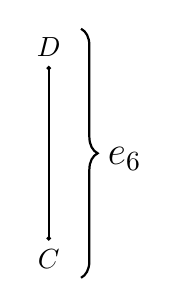
\begin{tikzpicture}[scale=1.25]
        \def\firstcoord{C}
        \def\secondcoord{D}
        \path coordinate (\firstcoord) at (0,0) coordinate (\secondcoord) at (0,1.73);
        \draw[thick] (\firstcoord) -- (\secondcoord);

        \draw[brace] (.3,-.4) -- node[blabel] {\Large $e_6$} (.3,2.13);

        \foreach \v/\position in {\firstcoord/below, \secondcoord/above} {
          \draw[fill=black] (\v) circle (0.5pt) node [\position=0.2mm] {$\v$};
        }
      \end{tikzpicture}
    \end{subfigure}\\\vspace{1.5cm}
    \begin{subfigure}{\linewidth}
      \centering
      \begin{tikzpicture}[scale=1.25]
        \path
        coordinate (A) at (-4,0)
        coordinate (B) at (-1.33,0)
        coordinate (C) at (1.33,0)
        coordinate (D) at (4,0);

        \foreach \v in {A,B,C,D} {
          \draw[fill=black] (\v) circle (2pt) node [below, yshift=-5pt] {$\v$};
        }
      \end{tikzpicture}
    \end{subfigure}\\\vspace{0cm}
    \caption{3-simplex and its basis faces. Note the 1, 4, 6, 4 relationship.
      Gotta love Pascal's 2-simplex!}
    \label{fig:circumscribed}
  \end{figure}
  \begin{enumerate}[label=(\arabic*)]\setcounter{enumi}{-1}
  \item $K$ is connected, so $\msf H_0(K) \cong \mb \zmod{2}$.
  \item Elements of $\msf B_1(K)$ are linear combinations of $\bdy[2]{A_1}$,
    $\bdy[2]{A_2}$, $\bdy[2]{A_3}$, and $\bdy[2]{A_4}$.
    \begin{itemize}
    \item Given any single edge, adding $A_i$
    \end{itemize}
  \item $\msf Z_2(K) = \set{\mb 0, A_1 + A_2 + A_3 + A_4} = B_2(K) \cong
    \zmod{2}$, so $\msf H_2(K) \cong \mb 0$.
  \item $\msf H_3(K) \cong \mb 0$.
  \end{enumerate}
\end{solution}
\begin{problem}[16.10]
  Let $K$ be a triangulation of a 2-sphere that consists of the proper faces of
  a 3-simplex. Compute $\msf H_n(K)$ for each $n$.
\end{problem}
\begin{solution}
  Proceed as before for $k=0,1$. For $k=2$, note $\msf B_2(K) \cong \mb 0$.
  Hence, $\msf H_2(K) \cong \zmod{2}$.
\end{solution}
\begin{definition}
  Let $K$ be a simplicial complex with $\abs{K} \subset \RR^n$. A point $x
  \not\in K$ can \emph{see} $K$ if any ray from $x$ intersects $\abs{K}$ at most
  once (as seen in the following diagram).
\end{definition}
\begin{figure}[H]
  \centering
  \begin{subfigure}{.49\linewidth}
    \centering
    \tdplotsetmaincoords{70}{80}
    \begin{tikzpicture}[tdplot_main_coords, scale=2]
      \path
      coordinate (A) at (0,0,0)
      coordinate (B) at (2,0,0)
      coordinate (C) at (1,1.732,0)
      coordinate (x) at (1,.577,1.733);

      \fill[red!30!white,draw=black] (A)--(B)--(C)--cycle;

      \path
      coordinate (P1) at ($.2*(A) + .5*(B) + .4*(C)$)
      coordinate (P2) at ($.3*(A) + .5*(B) + .2*(C)$)
      coordinate (P3) at ($.2*(A) + .2*(B) + .6*(C)$)
      coordinate (P4) at ($.7*(A) + .2*(B) + .1*(C)$);

      \foreach \v in {P1,P2,P3,P4}{
        % Take the difference and go slightly past it
        \draw[-latex,dashed] (x) -- ($1.3*(\v) - .3*(x)$);
        \draw[fill=black] (\v) circle (0.5pt);
      }

      \foreach \v in {A,B,C}{
        % Take the difference and go slightly past it
        \draw[-latex,dashed] (x) -- ($1.2*(\v) - .2*(x)$);
        \draw[fill=black] (\v) circle (0.5pt);
      }

      \foreach \v/\position in {A/left,B/left,C/right,x/above} {
        \draw[fill=black] (\v) circle (0.5pt) node [\position=0.2mm] {$\v$};
      }
    \end{tikzpicture}
    \caption{$x$ sees a $2$-simplex}
  \end{subfigure}
  \begin{subfigure}{.49\linewidth}
    \centering
    \tdplotsetmaincoords{70}{80}
    \begin{tikzpicture}[tdplot_main_coords, scale=2]
      \path
      coordinate (B) at (2,0,0)
      coordinate (C) at (1,1.732,0)
      coordinate (x) at (.6,.577,1.533)
      coordinate (y) at (1.8,1.077,1.733);

      \draw (B)--(C);

      \path
      coordinate (P1) at ($.5*(B) + .5*(C)$)
      coordinate (P2) at ($.23*(B) + .77*(C)$)
      coordinate (P3) at ($.7*(B) + .3*(C)$)
      coordinate (P4) at ($.4*(B) + .6*(C)$);

      \foreach \v in {P1,P2,P3,P4}{
        % Take the difference and go slightly past it
        \draw[-latex,dashed,color=red!30!white] (x) -- ($1.3*(\v) - .3*(x)$);
        \draw[-latex,dashed,color=blue!30!white] (y) -- ($1.3*(\v) - .3*(y)$);
        \draw[fill=black] (\v) circle (0.5pt);
      }

      \foreach \v in {B,C}{
        % Take the difference and go slightly past it
        \draw[-latex,dashed,color=red!30!white] (x) -- ($1.2*(\v) - .2*(x)$);
        \draw[-latex,dashed,color=blue!30!white] (y) -- ($1.2*(\v) - .2*(y)$);
        \draw[fill=black] (\v) circle (0.5pt);
      }

      \foreach \v/\position in {B/left,C/right,x/above,y/above right} {
        \draw[fill=black] (\v) circle (0.5pt) node [\position=0.2mm] {$\v$};
      }
    \end{tikzpicture}
    \caption{$x$ and $y$ both see a $1$-Simplex}
  \end{subfigure}
\end{figure}

%%% Local Variables:
%%% TeX-master: "main"
%%% End: